%!TEX root = mb.tex



     
\section{Overview}\label{sec:overview}


\todo{say that we use service provider to mean cloud or smth else}

In this section, we present \sys's architecture, the threat model and applications supported.

\todo{in the header MB section, tell them to recall the example which provides a way to see them all together}
\todo{need to say somewhere that we are running Ipv6 internally -- we do not need it outside right?}

% TO CUT REMOVE: just mentino the figures and no need to explain 
\subsection{Aplomb/NFV architecture}

We recall the system setup in APLOMB  in Fig.~\ref{fig:sys-overview}.
We do not delve into the details, motivation, and gains of this setup, and refer the reader to~\cite{aplomb} for details. 
There are three parties: enterprise(s), the service provider (SP), and an external site providing
some service. The enterprise runs a gateway (GW) which sends traffic to a middlebox (MB) running in the cloud.
The service provider has a borderbox (we use this term instead of gateway to avoid
confusion) and a set of middleboxes. Traffic arriving at SP first reaches the borderbox and traffic leaving SP, leaves through the borderbox.  

There are two typical setups as in Fig.~\ref{fig:sys-overview}.  The first setup, in Fig.~\ref{fig:model1},  occurs when the enteprise communicates with an external site. The second setup occurs when the traffic is sent between two enterprises as in Fig.~\ref{fig:model2}. This allows for a more optimized and faster layout~\cite{aplomb} because  each enterprise has its own gateway.


\todo{we require a modification in this case, has to go back to gateway}

%The traffic from a client inside the enteprise passes through the gateway on the way out of the enterprise. The gateway redirects this traffic to the middlebox in the cloud.
%After performing various middlebox processing, MB returns the traffic to the gateway. The gateway finally sends the traffic to the external site. 



%Traffic from a client in enterprise 1 passes through the gateway of this enterprise, then it goes  to the middlebox in the cloud, which after processing the traffic, sends it to the gateway of the second enterprise, and the traffic finally arrives at the receiver. This setup allows for better latency, as discussed in~\cite{aplomb}.




\todo{this  HTTP header values on a packet-by-backet basis without requiring any TCP bytestream reconstruction.table is a bit confusing -- better say whether they are dpi or header, also maybe what is field it operates
on, and what it encrypts, whether H or DPI, put section near the name; also in intro make the dpi vs header distinction already} 


\subsection{Threat model}

The goal of \sys is to protect the privacy of the traffic against an attacker at the cloud 
(cloud employee, or hacker gaining access to cloud machines). 
We consider a strong cloud attacker, one that has gained access to {\em all the data on the cloud}.
This includes any traffic and communication the cloud receives from the 
gateway, any old logged information, cloud state, and so on. Nevertheless, we assume that 
the cloud provides good service and runs middlebox functionality correctly.  We are only concerned with 
the traffic's confidentiality.

We assume that the gateways are trusted. They do not leak information.


Some middlebox functionalities (such as intrusion detection or exfiltration detection) have a threat model
of their own regarding the client and the server. For example, intrusion detection assumes that 
the client or the server could misbehave and try to mount an attack, but at most one of them misbehaves~\cite{Bro}  
(indeed, if both misbehave, they can send attack traffic to each other encrypted with a shared symmetric key and fundamentally
no one can detect such an attack).  We preserve all these threat models unchanged. These applications rely
on the good behavior of the middlebox to detect attacks in these threat models. Since we assume the middlebox executes
these functions correctly and \sys preserves the functionality of these middleboxes, 
these threat models are irrelevant to the protocols in \sys, and we will not discuss them again. 


\subsection{Goals at gateway}

\todo{don't change on upgrades of software}
\todo{say that we accomplish them}
\todo{no state per connection}
\todo{not much work, although much is config and version maintenance }
\todo{use this in tex?}
\todo{could have ssl encryption too}
\todo{gateway does encryption and ipv6 -- }
\todo{why ipv6 because it is needed}
% Firewalls from different vendors may vary significantly in terms of rule syntaxes and organizations. However,
% in general both hardware and software firewalls have a few interfaces. Both ingress and egress of an interface 
% can be associated with an access control list (ACL). Each ACL has a number of rules, possibly in the form 
% <action, protocol, src ip, src port, dst ip, dst port>. Without loss of generality, we take \texttt{pf}, the 
% default firewall under BSD, as an example to illustrate how \sys works with firewalls. Figure \ref{fig:fwrule1} 
% shows an example of \texttt{pf} rules. 
\todo{no more need for the borderbox}

\subsection{\sys overview}


\begin{figure}[t!]
\centering
  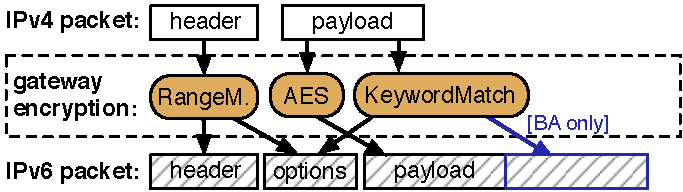
\includegraphics[width=2.0in]{fig/packet.pdf}
\caption{Packet encryption at the gateway. Patterned squares indicate encrypted data. \label{fig:sys-overview}}
\end{figure}


\todo{explain that the borderbox helps with updates in encryptions and with decryption of schemes that cannot be decyrpted}
\todo{perhaps indicate the borderbox in the figure}



\begin{figure*}[t!]
\centering
  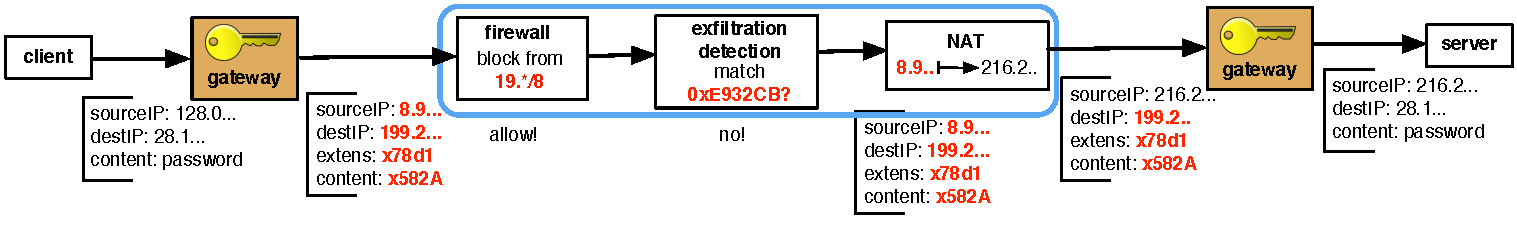
\includegraphics[width=6.7in]{fig/packetpath.pdf}
\caption{Example of packet flow through a few middleboxes. Red indicates encrypted data. \label{fig:sys-overview}}
\end{figure*}



To protect privacy of the traffic, \sys encrypts all traffic passing through the middlebox at the cloud. 
As in Fig.~\ref{fig:sys-overview}, the gateway has a secret key $k$; in the setup with two gateways, they share
the same secret key. The gateway encrypts all traffic going to the middlebox in the cloud using \sys's protocols.
The middlebox in the cloud processes {\em encrypted traffic} using \sys's protocols. 
After the processing, the middlebox
will produce encrypted traffic which it sends back to the gateway. The gateway decrypts the traffic using the key $k$.

Throughout this process, MB handles only the encrypted traffic and never gets the decryption key. This ensures
that an attacker that steals all data from the cloud, will only see encrypted traffic and hence protects the privacy of the 
traffic. 
\sys encrypts IP addresses, ports, and the payload of the packet, thus protecting the privacy of all these parameters. 
Middleboxes at the cloud operate over the encrypted values in each packet, and do not have access to the decrypted data.

\sys enables encrypted operation for {\em all} typical middleboxes in outsourcing scenarios, despite substantial differences in how the middleboxes operate, what packet data they access, and whether they modify or merely observe packets.
  We classify middleboxes in to two broad categories based on the type of data they access: {\em header-only} middleboxes and {\em bytestream-aware} middleboxes.
  Some middleboxes are `header-only' middleboxes: they operate over packet headers (\eg{}, IP or TCP headers) on a packet-by-packet basis.
Examples of header-only middleboxes include IP Firewalls and Network Address Translators (NATs).

  Other middleboxes are `bytestream-aware.' These middleboxes operate over a TCP bytestream -- the concatenation of all {\it payloads} -- and hence must keep substantial state per connection.
  For example, many Intrusion Detection Systems (IDS) are bytestream-aware; in order to detect attack signatures that span across multiple packets they keep a buffer which with copies of each payload it has forwarded.
  It uses these payloads to to reconstruct the TCP bytestream, just as the client will observe at the application layer; the IDS can then scan this bytestream for malicious substrings.
  Web proxies are also bytestream-aware; rather than keeping a copy of packets the proxy forwards, the proxy performs {\it session termination}. 
  When a client opens a new HTTP connection, a typical proxy will capture the client's SYN packet and open a new connection to the client, as if it were the web server the client wished to connect to. 
  The proxy also maintains second connection in the background to the original web server, as if it were the client. 
  Session termination allows the proxy to cache entire images (which usually span multiple packets) and respond to client requests with cached data as if it were the server.
  In Table~\ref{tab:apps-ops}, we list each middlebox, the cryptographic tools used to encrypt it, and whether it is a bytestream-aware (BA) or header-only (HO) middlebox.

  As we will see, to support header-only middleboxes, the \sys gateway can also operate in a header-only fashion, encrypting each header field (\eg{}, IP address, port number) independently.
  However, to support bytestream-aware appliances, the \sys gateway also needs to be be bytestream aware, in order to encrypt the concatenation packet payloads.
  The one exception to this rule -- that header-only middleboxes can be served by a header-only gateway, while bytestream-aware middleboxes require a bytestream-aware gateway -- is web proxying.
  Proxies are bytestream-aware, but can be served by a header-only middlebox when they do not allow pipelined requests.
  As we will discuss in \S\ref{sec:proxies}, the gateway can encrypt the HTTP header values on a packet-by-backet basis without requiring any TCP bytestream reconstruction so long as HTTP pipelining is not enabled. 

\todo{make clear not outsourcing because of performance}

{\bf Miscellaneous TODOs:}

- the key is called k

- some of the paragraphs above are redundant with intro perhaps

-maybe the overall packet structure here or should this bein systems implementation? 

- need to discuss what happens to SSL connections here; what if the client initiates one? the gateway can no longer
encrypt things

-- handling two gateways with non-determinism

-- goals on the gateway, gateway only needs to know which apps are running, note that in our design
it does not depend on the version, etc. 

-- have a way to show that what the gateway does is generic 
   
-- somewhere we need to discuss goals regarding the gateway

-- why we choose certain operations

which app for which operation


- need to discuss somewhere the above goals from the gateway
%A LOT OF SYSTEMS BUILDING

- security guarantees:

- why we choose certain operations

- Need to summarize somewhere "overall" security

- Somewhere we need to say that range match info leaks for header and keyword match for content. In some sense, these are minimal. 

